\documentclass{beamer}
\usepackage{amsmath}
\title{Resource Access Planning:  Healthcare - Electricity}
\author{Chris Natali}
\institute{Modi Labs at Columbia University}
\date{May 22, 2013}
\begin{document}

\begin{frame}{Development Planning}

  Improving Access to Resources

  \bigskip 

  What: 
  \begin{itemize}
  \item[] Healthcare:  Clinics, Hospitals, Doctors, Nurses...
  \item[] Education:  Schools, Teachers, Classrooms...
  \item[] Water:  Wells, Pumps, Taps...
  \item[] Electricity:  Generators, Transformers, LV/MV line...
  \end{itemize}
 
  \bigskip 

  Where: 
  \begin{itemize}
  \item[] Access is limited
  \item[] Sub-Saharan Africa (minus South Africa)
  \item[] India, Indonesia
  \item[] Rural regions
  \end{itemize}


\end{frame}


\begin{frame}{Process}

  How: 
  \begin{itemize}
  \item[] Identify problem
  \item[] Collect data:  From existing sources, Formhub, other tools
  \item[] Frame it in economic terms (supply, demand)
  \item[] Analyze "gaps" in supply 
  \item[] Develop plan to fill the gaps
  \end{itemize}

\end{frame}

\begin{frame}{Health Clinic Access Initial}
  \includegraphics[width=4.5in,height=2.75in]{../diagrams/nigeria-healthcare-initial_6.png}
\end{frame}

\begin{frame}{Health Clinic Access Optimized}
  \includegraphics[width=4.5in,height=2.75in]{../diagrams/nigeria-healthcare-optimized_16.png}
\end{frame}

\begin{frame}{Electrification Planning}
  
  Sea Urchin Story (Healthcare is more effective with Electricity)

  \bigskip 
  Inputs: 
  \begin{itemize}
  \item[] Supply:  Existing grid
  \item[] Demand:  Settlements to be electrified
  \item[] Model Parameters:  Generation, Distribution costs, Growth/Demand curves
  \end{itemize}

  \bigskip 

  Outputs: 
  \begin{itemize}
  \item[] Electrification selection per settlement (Solar, Diesel, Grid)
  \item[] Costs (settlement and regional level)
  \end{itemize}

\end{frame}

\begin{frame}{NetworkPlanner Liberia}
  \includegraphics[width=4.5in,height=2.75in]{../diagrams/network-planner-liberia.png}
\end{frame}

\begin{frame}{Data Collection System}
  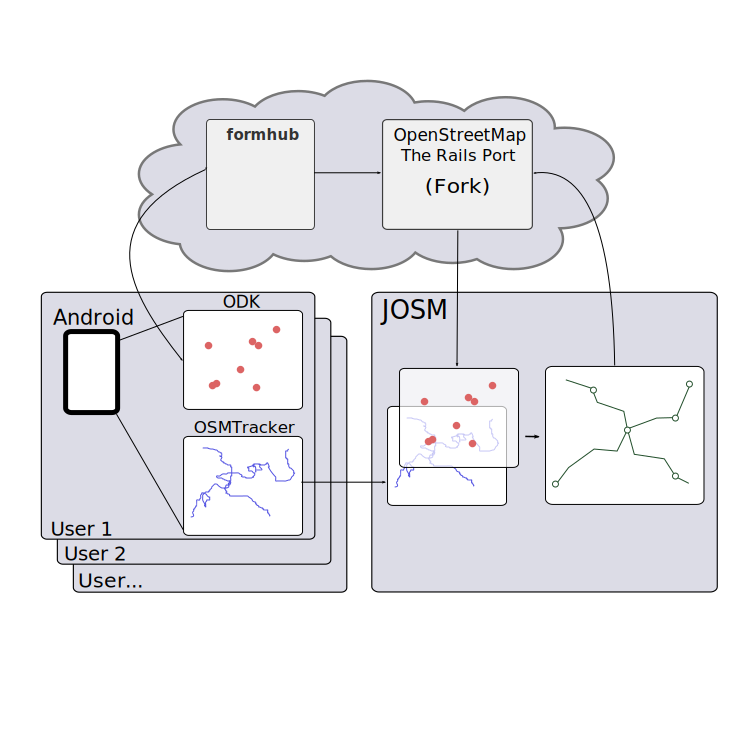
\includegraphics[width=4in,height=3in]{../diagrams/gridmaps-design.png}
\end{frame}

\begin{frame}{Results}

  Numbers:
  \begin{itemize}
  \item[] 700 km of new mv grid data captured
  \item[] Average of about 50 km of mv grid captured per day
  \item[] 7000 km of mv grid managed 
  \end{itemize}
  
\end{frame}

\begin{frame}{Data Collection Map}
  \includegraphics[width=4.5in,height=2.75in]{../diagrams/gridmaps-indo.png}
\end{frame}

\begin{frame}{The End}

  \begin{itemize}
  \item[] Our Lab:  modi.mech.columbia.edu
  \end{itemize}
 
\end{frame}
\end{document}
